\chapter{Design and architecture}
\label{ch:design}
% Intro per chapter, refer to problem definition each time, where are we now, what now (for reader)
% Why this chapter
% Paragraphs
% Conclusion of contents of this chapter
% Link to next chapter

We now present a design to address the challenges and utilize the opportunities of working on a mobile device as put forward in the previous chapter.
First in terms of functionality and other requirements, second the overall system architecture.

Previous attempts at designing a mobile version of Tribler failed to properly separate re-usable components.
This resulted in unmaintainable code and increased difficulty in testing.
We use a top down approach to come to a high level system architecture and in determining the reusable components or the current Tribler application.
% What is the gap?
Some functionality of Tribler has been shown to work on Android before \cite{bsc1,2,3}.
Our design will fill in the gap of connecting the pieces of the grand puzzle to make Tribler fully work on mobile.


\section{Functional requirements}
% Functional level
% Function design
%Product design involves determining the objectives of the system. Central questions in this process are “what is feasible?”, “what is required?” and “what functions need to be fulfilled by the system?” It is a strategic decision process and it will be termed the function design 
%Function design distinguishes between innovation and improvement. Improvement usually only concerns the reorganisation or reengineering of an existing system, which implies a rearrangement of existing functions or a different interpretation of these functions. Innovation concerns the extension, reduction or modification of functions due to the introduction of new technology, resources and/or organisation.

%inputs, commands and conditions
%outputs, conditions
%store, reuse data, backup
%computations
%timing and synchronization

Because of the ubiquity of smart-phones with built-in camera one is always at hand and ready to record.
Such mobile devices are much more manageable than for example laptops with built-in camera that Tribler has been capable of running on in the past.
No opportunity has to be missed due to hassle of getting a dedicated camera and transferring the recording to a connectible device afterwards.
Therefore the camera built-in the mobile device should be used to record video or photographs with Tribler.
The usability of Tribler as a content generating tool is greatly improved by this. 

Publishing content should be one simple step for the user to perform, especially right after creating new content.
Every user must be able create his/her own channel in Tribler to publish their content, just like channels in YouTube, directly from the mobile device.
Newly discovered channels and content may be added to the GUI without user interaction.

To easily share your own channel with others the id could be transferred via NFC from device to device.
With just one-click-confirmation it should be send, and the receiving device must then be able to subscribe to this channel and start discovering the contents automatically right away.
Because this may require both devices having Tribler installed, it also must be able to share the installation package via Bluetooth or WiFi without any prerequisites on the receiving device.

Self-created content must be stored on the internal memory and processed automatically on the mobile device itself in order to avoid dependency any external processing unit.
This includes the creation of .torrent files required to share content via the bit-torrent protocol.

\begin{enumerate}[label=A\arabic*.,ref=req. A\arabic*]
	
	\item The implementation must be capable of publishing videos to other devices with and without an Internet connection.
	\item The implementation must be capable of recording videos.
	\item Any video available on the device must be directly publishable. %acquisition
	\item The implementation must enable a user to create a channel.
	\item The implementation must enable the owner of an existing channel to edit it.
%	\item The implementation should enable the user to add torrents by url
	\item The implementation must enable creating a torrent file from a file available on the device.
	\item A user must be able to manually configure the Tribler configuration on the device.
%	\item The configuration of Tribler core must be stored separately from the data in a human readable form to enable users to alter it with an external editor.
	\item The implementation must support video playback.
	\item The implementation must support all other Tribler functionality not mentioned above.
%	\item The app must enable the user to search local and remote content in parallel.
%	\item The app must support Multichain
%	\item The app must support streaming video playback
%	\item The app must support a family filter
%	\item The app must support the content classification algorithm of Tribler
	
\end{enumerate}


\section{Non-functional requirements}

Due to the challenges and opportunities as described in Section \ref{ch:tribler_mobile}, we define the following non-functional requirements:

\begin{enumerate}[label=B\arabic*.,ref=req. B\arabic*]
	
	\item \label{rq1}The mobile device must be capable of running Tribler independently.
	%re-usability
	\item The implementation must incorporate the existing Tribler Python core and the required C/C++ libraries.
	%technology to be used: programming language, db
	%resource usage
	\item The implementation may not exceed 512MB of RAM usage while running.
	\item The implementation must be capable of running on ARMv7 or compatible mobile processors.
	%computing platform: min. system specs and features, api level
	\item The implementation must support WiFi, Bluetooth and NFC peer-to-peer features.
	\item The implementation must utilize the built-in camera for recording videos.
	\item The mobile device must be connectible via WiFi or mobile data connection
	%response time
	\item Search results ought to appear in less than 1 second for local content.
	%throughput
	% Design for portability
	\item The implementation must be distributed as a single installable container.
%	\item The app must communicate with the JSON REST API of the Tribler core.
	\item The implementation must be able to keep running in the background even if the user is not actively using it.
	\item All processing tasks must be performed asynchronously.
	\item The user must be able to interact with the implementation via a graphical user interface (GUI).
	\item All ongoing tasks must be indicated as such in the GUI.
	\item The GUI must stay responsive to the users' input while performing a background task.
	\item The GUI must stay responsive to the users' input while presenting large amounts of data on screen.
	%reliability
	\item If invalid input is provided by the user through the GUI the user must be asked to correct the input.
	%availability
	%recover from failure
	\item If a recoverable error occurs, the implementation must automatically retry.
	\item If an exception occurs, the user must be able to restart Tribler.
	\item Upon restarting, the implementation must return to a working state.
	%maintainability and enhancement
	\item The entire build tool-chain must be integrated on the build server of Tribler. % for continuous integration. To keep the project maintainable
%	\item All existing tests, except platform specific and desktop GUI tests, must be performed for every build.
	\item As much code as possible must be covered by tests.
	% Keep the level of abstraction as high as possible
	\item The implementation must be agnostic to version differences of supported platforms and operating systems.
	% reuse of expertise
	\item The user interface design must follow established best practices.%, like Google's "material design".
	% reuse of standard designs and algorithms
	% reuse of libraries of classes or procedures, of of powerful commands built into languages and operating systems
	% reuse of frameworks
	% reuse of complete applications
%	\item Re-use an existing library or preferably an entire app, instead of re-implementing multi-media functionality and player interface.
	% Anticipate obsolescence
	% Design for testability
%	\item The GUI must be able to be tested separately from the back-end.
%	\item The API must be able to be tested independently.
%	\item The API should be consistent.
%	\item The API should be clearly documented for other developers.
	% Design defensively
	\item The implementation must be attack-resilient.
	% Internationalization
%	The GUI should support other languages to be added without changing source code.
	% Resource usage
%	The separation of front-end and back-end should not lead to resources being loaded into memory twice or anything of that matter.
	% Usability
%	Make use of universally recognizable icons that are native to the platform UI.
%	The responsiveness of the GUI must not be significantly impacted by the amount of data presented on screen.
%	The responsiveness of the GUI must also not be significantly impacted by the amount of computational work, or otherwise, done in the background.

\end{enumerate}


\section{System architecture}
% Design level

The requirements dictate how the system architecture of Tribler on mobile devices will take shape.
% Increase re-usability where possible
The proposed architecture as shown in Figure \ref{fig:system_architecture_design} is specifically designed for maintainability and clearly separates components with a distinct responsibility.

\begin{figure}[H]
	\centering
	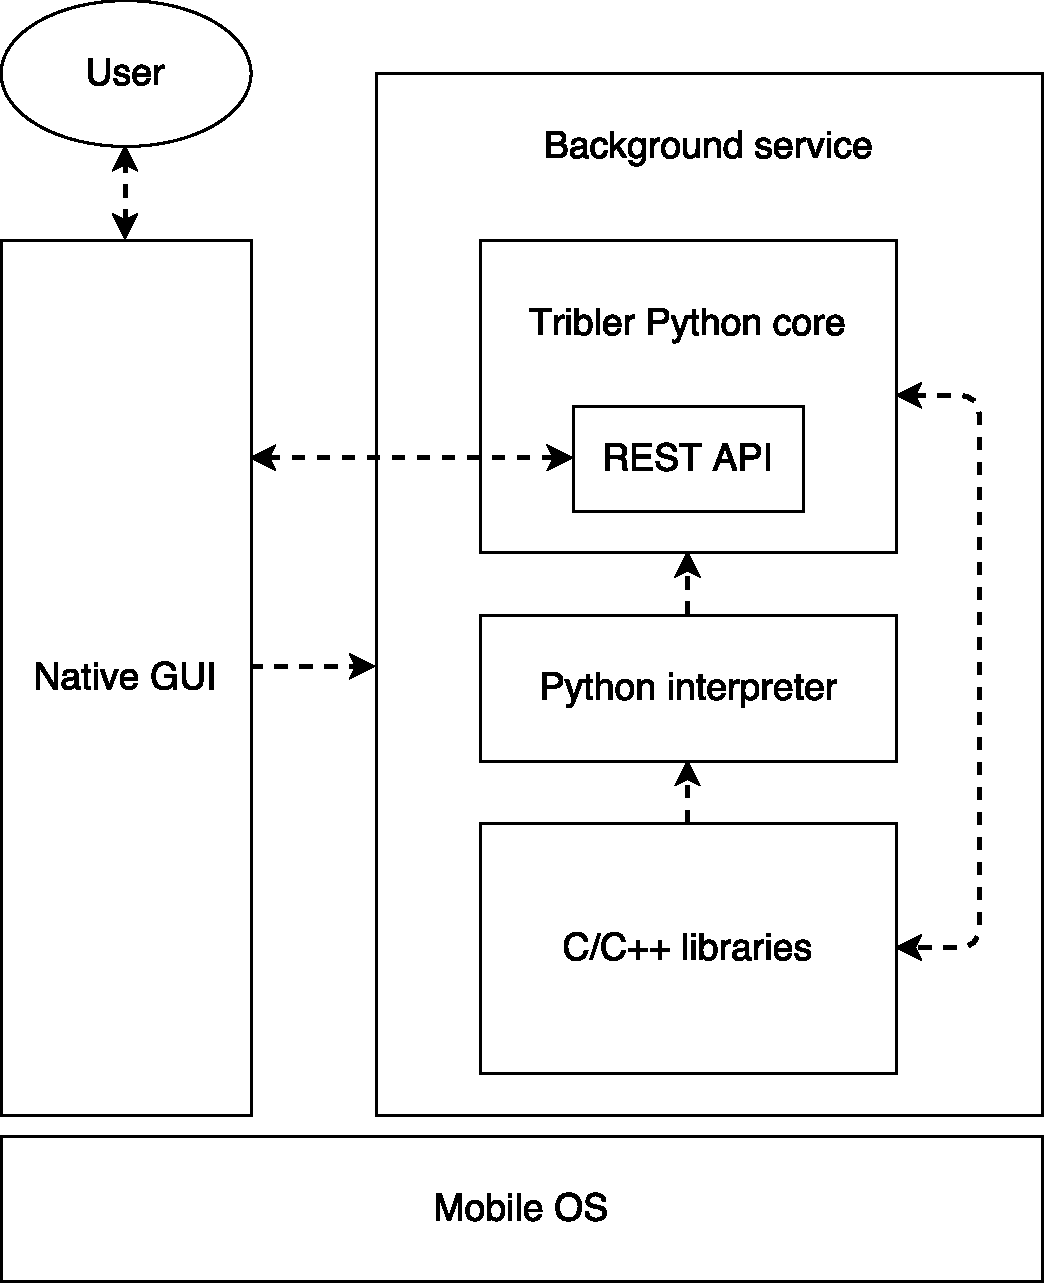
\includegraphics[width=0.5\textwidth]{system_architecture_design}
	\caption{System architecture}
	\label{fig:system_architecture_design}
\end{figure}

The requirement of re-using the Tribler Python core and its C/C++ dependencies requires the architecture to incorporate these as is.
As a consequence, a Python interpreter must be added to the design as well.
Since mobile platforms are not required to support running Python code natively, but the application must be distributed as a single installable package and run independently (\ref{rq1}), the interpreter is packaged inside the application.
% Reuse existing designs and code where possible
% What are the existing modules we re-use?
%Having separated the GUI from the back-end, we can easily re-use the Tribler core and replace the outdated wxPython GUI with something modern.
The user must interact with the implementation via a GUI \ref{}.
As such a GUI is not part of the Tribler core, it has to be included separately in the design.

The requirements on asynchronous communication and responsiveness \ref{}require the decoupling of the GUI from the back-end. % async front-back means rest api
% Design for flexibility / adaptability
A separate GUI can be made and optimized for any specific platform and target device. % native user interface interaction.
For instance, a design can be made for large surface displays and another one for small touch-screens, like a smart-phone.
This leads to the design choice of creating an API that allows for a common interface across all platforms to let the GUI communicate with the existing Tribler core.

The API will yield a more maintainable solution than previous attempts to bring Tribler to mobile devices \cite{bsc1,2,3} that did not include such an API.

% Divide and conquer
%Recent refactoring of the Tribler code \cite{thesis_martijn} has divided functionality into core modules.
% Increase cohesion where possible
% Reduce coupling where possible
%The purpose of this was to increase cohesion inside modules and the core, and reduce coupling between modules where possible.
%This makes porting the core and individual modules easier.

